

\section{The need to combine resolution and precision}

Traditional data reduction techniques work in either resolution space or precision space
exclusively. They truncate either the last few levels in a multi-resolution representation of the
data, or the last few low-ordered bits, but rarely both. Our aim in this section is to show that
significant gain can be achieved when one combines both dimensions of data reduction. To do so, we
construct and compare different ways to order the bits of a data set so that bits that have higher
impact on the error (in regards to a metric of interest) appear earlier. We call each ordering a
\emph{stream} of bits. The idea is that, if the data is streamed to a receiver using a bit ordering
that is optimized for a certain metric, the receiver would be able to perform analysis tasks
pertaining to that metric as soon as possible, while incurring minimal error.

Streams are not constructed from raw data bits, but from a representation in which every bit can be
associated with a resolution level and a bit plane. We use the CDF5/3 wavelet transform [CITE] to
decompose the domain into resolution levels (also known as subbands). To handle precision in a
unified way, we quantize the resulting wavelet coefficients to $16$-bit signed integers, which are
then converted to negabinary form [CITE]. In each subband, negabinary coefficients are grouped into
groups of $g \times g$ in 2D, and each group is divided into \emph{chunks}. A chunk contains a
single bit plane of all coefficients in the group. For performance reasons, we do not stream one bit
at a time, but always one chunk at a time (a typical chunk size used in this paper is $4 \times 4 =
16$ bits). This constraint is reasonable because in practice, data is almost never read or written
bit-by-bit.

Of the streams to be compared, one proceeds strictly from coarser to finer resolution levels
(\emph{by level}), one proceeds stricly from higher-ordered to lower-ordered bit planes (\emph{by
bit plane}), and one combines resolution and precision (\emph{by wavelet norm}). The \emph{by
levels} stream is designed to represent the way data is read in traditional multi-resolution
techniques such as those based on subsampling [CITE], octrees [CITE], or wavelets [CITE]. The
\emph{by bit plane} stream represents techniques that truncate data in precision such as zfp [CITE].
The \emph{by wavelet norm} sort chunks in decreasing order of $\norm{W_l}_2 \times 2^b$, where $l$
and $b$ are a chunk's subband and bit plane, and $W_l$ is the wavelet basis function at subband $l$.
These three streams are data-independent. We also include in the comparison two data-dependent
streams, namely \emph{resolution-adaptive} and \emph{fully adaptive}. In the
\emph{resolution-adaptive} stream, chunks are ordered so as to minimize peak-signal-to-noise ratio
(PSNR [CITE]), with one constraint: every wavelet coefficients must come in full precision (in other
words, chunks of the same group are streamed together). The \emph{fully adaptive} stream orders
chunks to minimize PSNR the same way, but without any constraints. Both streams are constructed
using the greedy algorithm discussed in Section [REF].

For each stream, everytime a chunk is received, the data is reconstructed at full resolution using
only the chunks received so far. An error value is then computed, depending on the metric in used
(e.g., PSNR, histogram error, isocontour error, etc). For the $512 \times 512$, double-precision
data set \emph{Magnetic} [REF], Figure \ref{fig:motivation} compares the five streams in
PSNR relative to the original (unquantized) data. We note that for this particular comparison,
chunks containing only leading zero bits are removed for all streams, to mimic the effect of entropy
compression in practice.

\begin{figure}
	\centering
	\subcaptionbox{Magnetic}
	{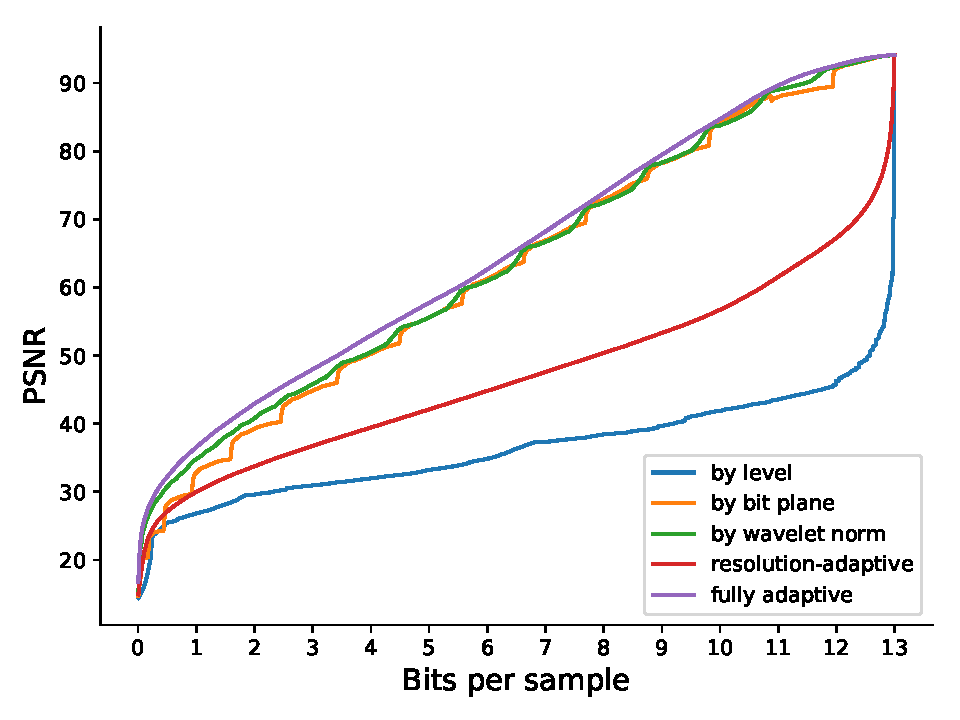
\includegraphics[width=0.44\linewidth]{img/motivation/magnetic-motivation.pdf}}
	\subcaptionbox{Boiler-O2}
	{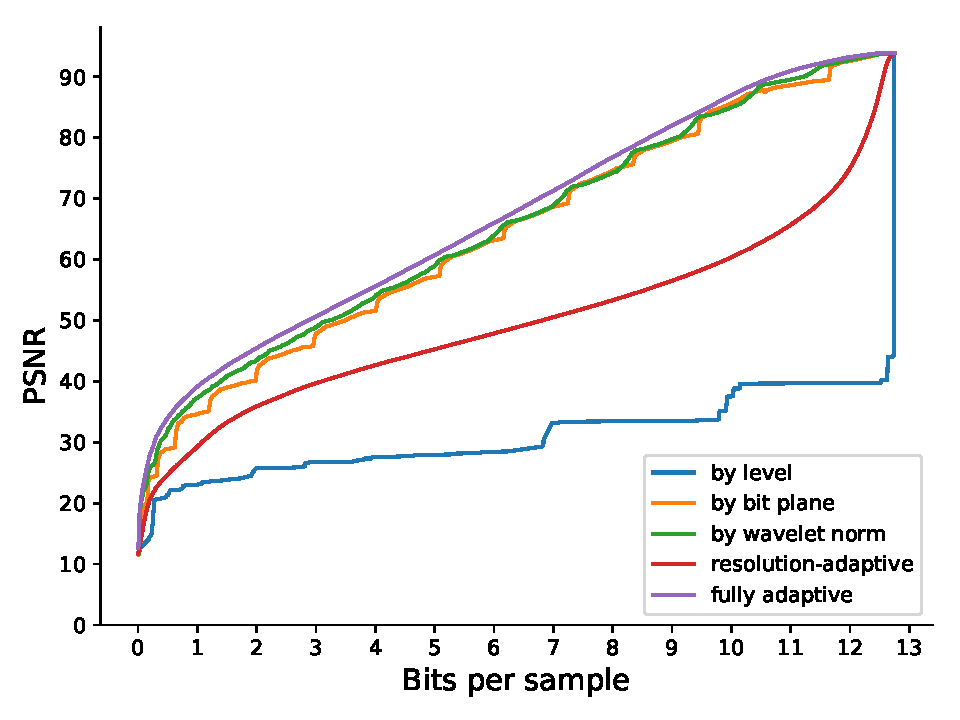
\includegraphics[width=0.44\linewidth]{img/motivation/boiler-oh-motivation.pdf}}
	\subcaptionbox{Flame-OH}
	{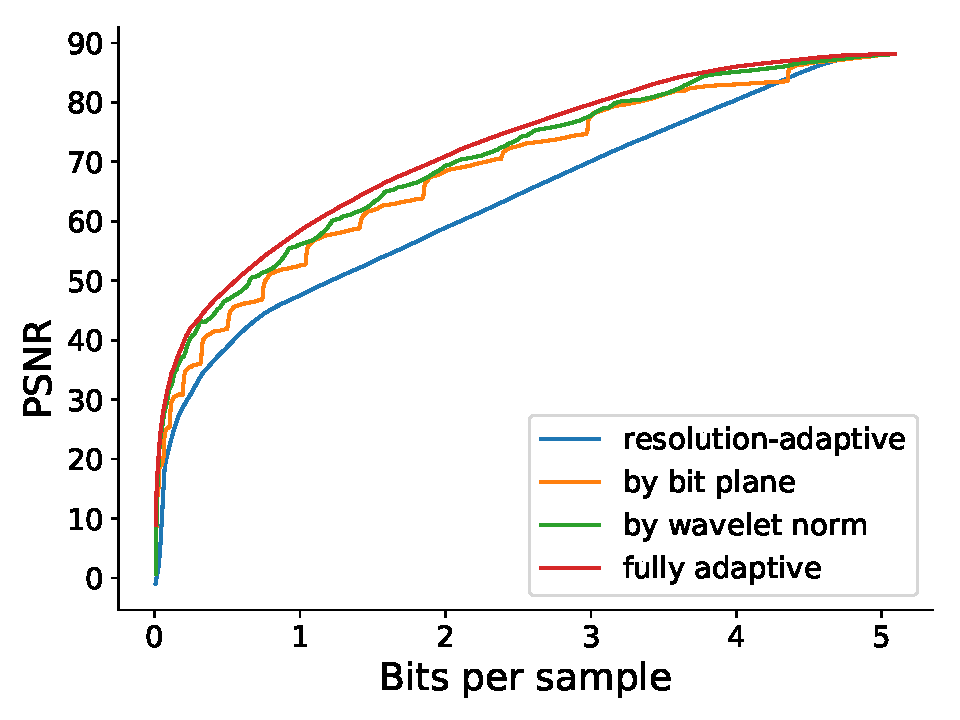
\includegraphics[width=0.44\linewidth]{img/motivation/kflame-oh-motivation.pdf}}
	\subcaptionbox{Miranda-diffusivity}
	{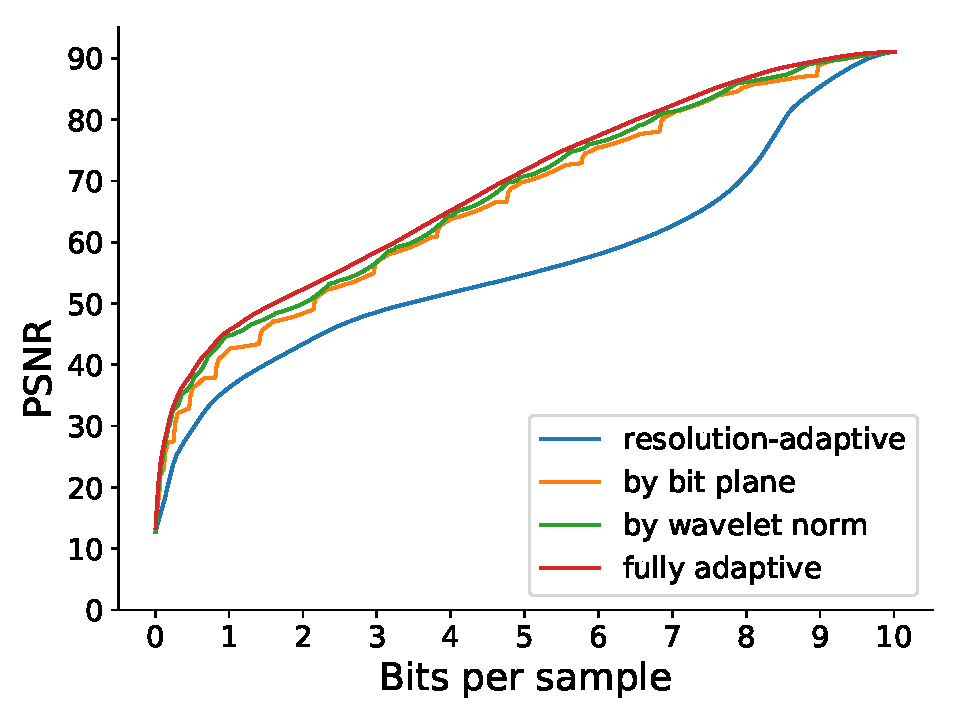
\includegraphics[width=0.44\linewidth]{img/motivation/miranda-diffusivity-motivation.pdf}}
	\caption{PSNR comparison of streams that are by resolution exclusively (\emph{by level} and
	\emph{resolution-adaptive}), by precision exclusively (\emph{by bit plane}), and by both combined
	(\emph{by wavelet norm} and \emph{fully adaptive}). Higher is better. A 20 dB increase in PSNR
	approximately translates to one more decimal digit of accuracy.}
	\label{fig:motivation}
\end{figure}

It can be seen from Figure \ref{fig:motivation} that the streams that combine resolution and
precision (\emph{by wavelet norm} and \emph{fullly adaptive}) perform the best, either among the
data-independent streams, or the data-dependent ones. This is true across all four data sets shown,
and for all other data sets in our experiments. The \emph{fully adaptive} stream, can be thought of
as an empirical upper bound on how well any stream of the same data can perform in terms of PSNR. Of
the data-independent streams, \emph{by bit plane}approximates \emph{by wavelet norm}  well, but this
is true only when the error metric is PSNR. In the next section, we show that because of its greater
flexibility, the \emph{by wavelet norm} stream outperforms \emph{by bit plane} by a large margin
when it comes to computing an accurate histogram.

% \begin{figure*}[!htb]
% 	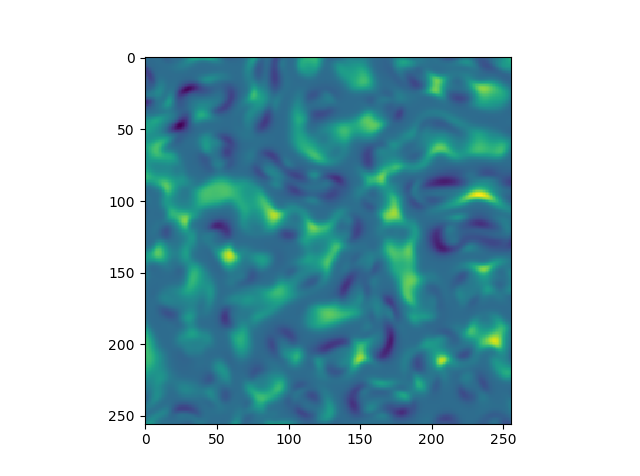
\includegraphics[width=0.33\linewidth]{img/dataset/miranda-viscosity.png}
% 	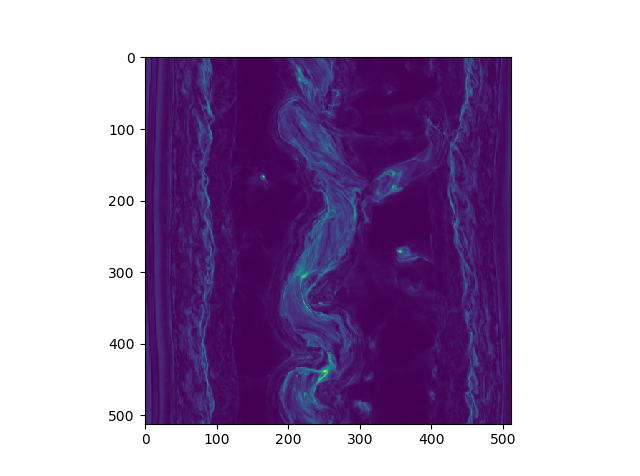
\includegraphics[width=0.33\linewidth]{img/dataset/magnetic.png}
% 	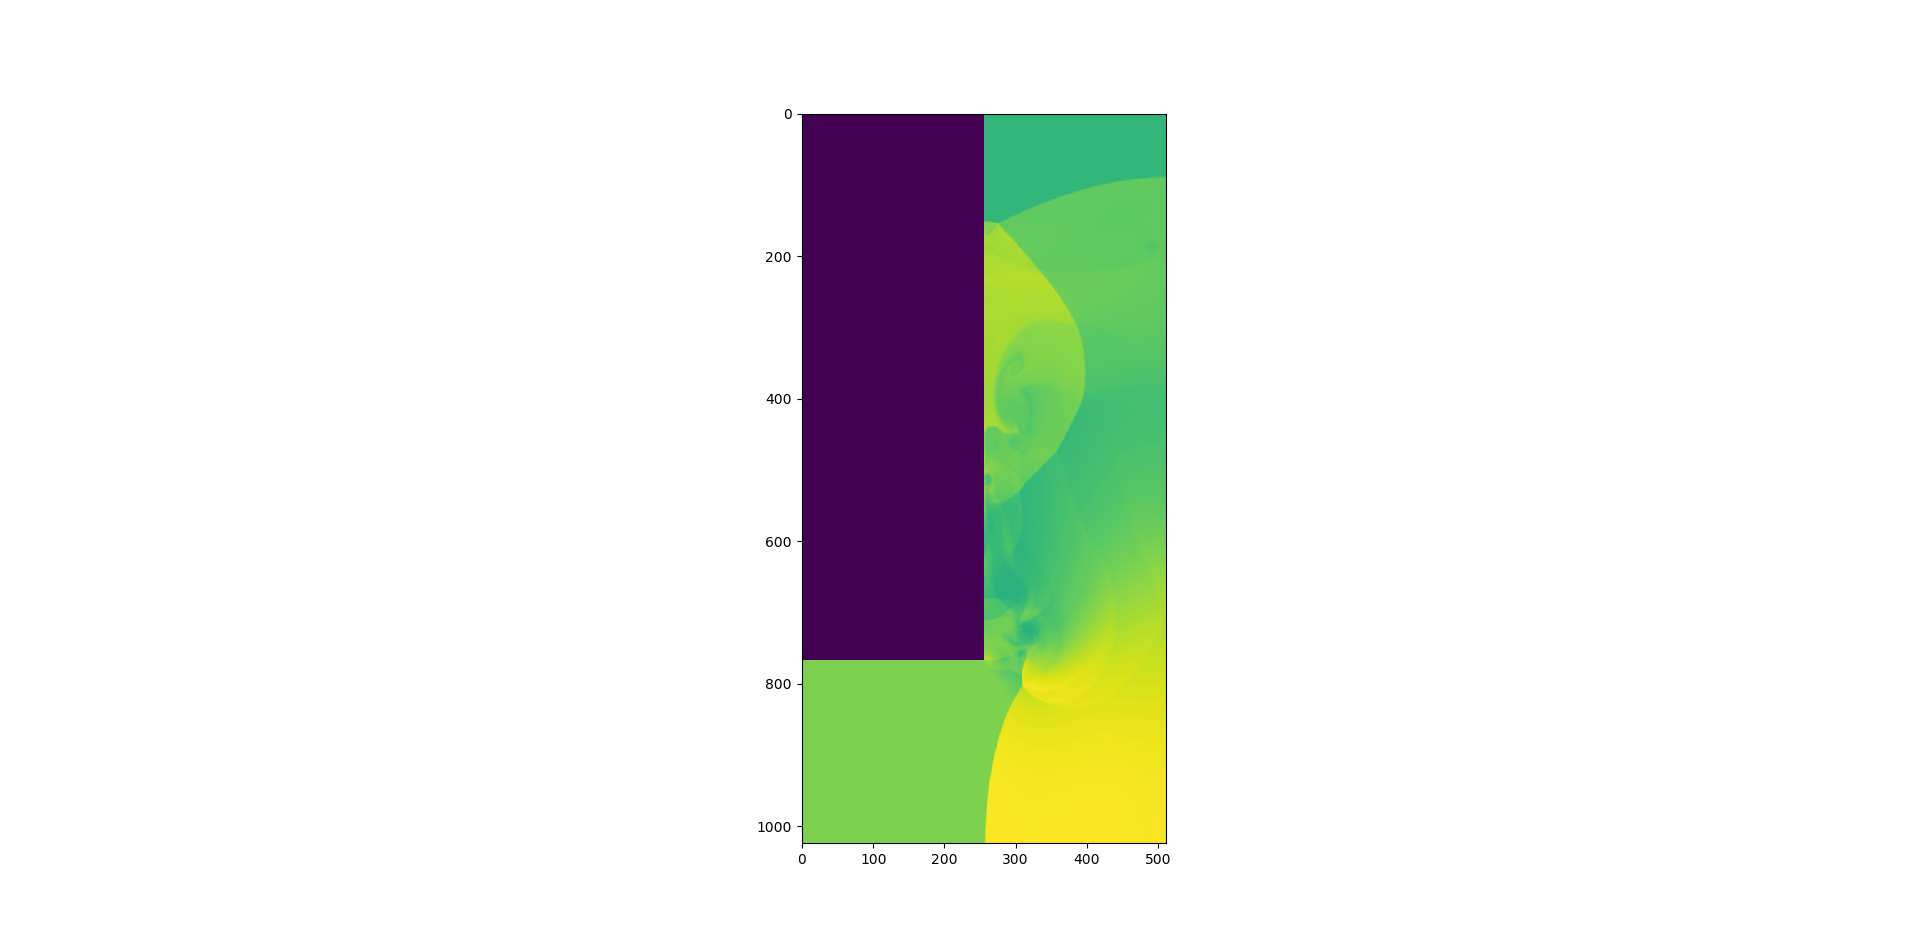
\includegraphics[width=0.33\linewidth]{img/dataset/euler2d.png}
% 	\caption{Left to right: Miranda viscosity field, magnetic reconnection, Euler 2d sharp front}
% 	\label{fig:datasets}
% \end{figure*}

% \begin{figure}[htb!]
% 	\centering
% 	\subcaptionbox{without skip leading zeros}
% 	{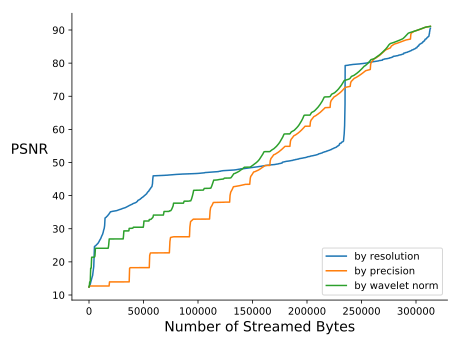
\includegraphics[width=0.4\linewidth]{img/independent/rmse-miranda-viscosity}}
% 	\subcaptionbox{with skip leading zeros}
% 	{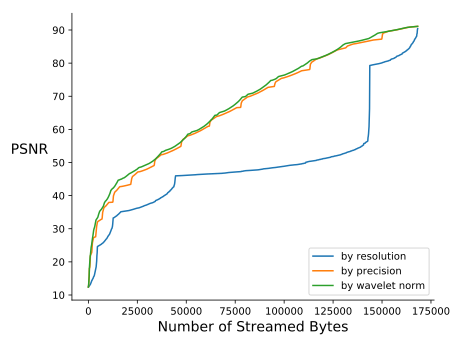
\includegraphics[width=0.4\linewidth]{img/skip-zeros/rmse-miranda-viscosity}}
% 	\caption {PSNR comparison between three streams: by bit-plane, by level, and by wavelet norm}
% 	\label{fig:psnr_traditional_vs_by_norm_viscosity}
% \end{figure}

% In the supplement materials, we show the same plot for the following datasets:
% \begin{enumerate}
%   \item Miranda viscosity (smooth and uniform)
%   \item Kingsnake (noisy and sparse)
%   \item Magnetic (tiny narrow lines)
%   \item Euler 2D (sharp front)
%   \item Enzo u (wide range)
% \end{enumerate}

\section{The need for task-optimized streams}
To test whether a stream that is suited to a certain task (function reconstruction, using PSNR as
the metric) also performs well in another (histogram computation), we compare the streams introduced
in the previous section using a histogram error metric that is the Earth Mover Distance (EMD)
[CITE]. The EMD measures how far the histogram of the reconstructed data is from the histogram of
the original data. We use 256 histogram bins in all experiments. The results are shown in Figure
\ref{fig:histogram-motivation}. Compared to Figure \ref{fig:motivation}, the \emph{by level} stream
is removed and two other streams are added: \emph{resolution-adaptive, EMD-optimized} and
\emph{fully adaptive, EMD-optimized}. The two new streams are analogous to their RMSE counterparts
(i.e., the two data-dependent streams in Figure \ref{fig:motivation}, now renamed to
\emph{resolution-adaptive, RMSE-optimized} and \emph{fully adaptive, RMSE-optimized}), but are
computed by greedily minimizing EMD instead of RMSE with regards to the groundtruth.

\begin{figure}
	\centering
	\subcaptionbox{Magnetic}
	{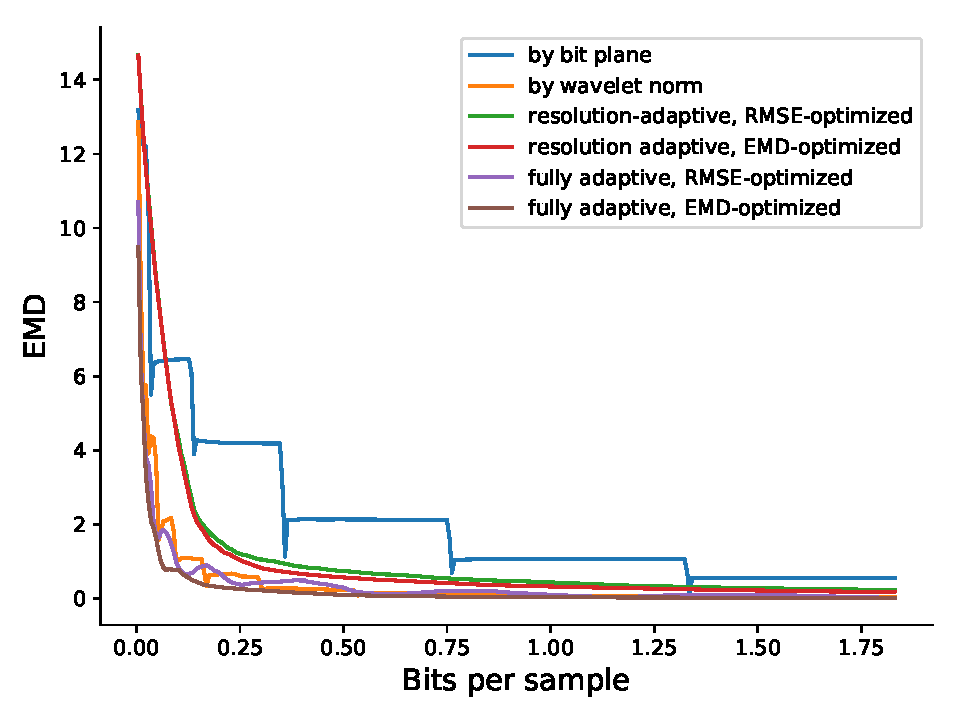
\includegraphics[width=0.44\linewidth]{img/motivation/magnetic-histogram-motivation.pdf}}
	\subcaptionbox{Boiler-O2}
	{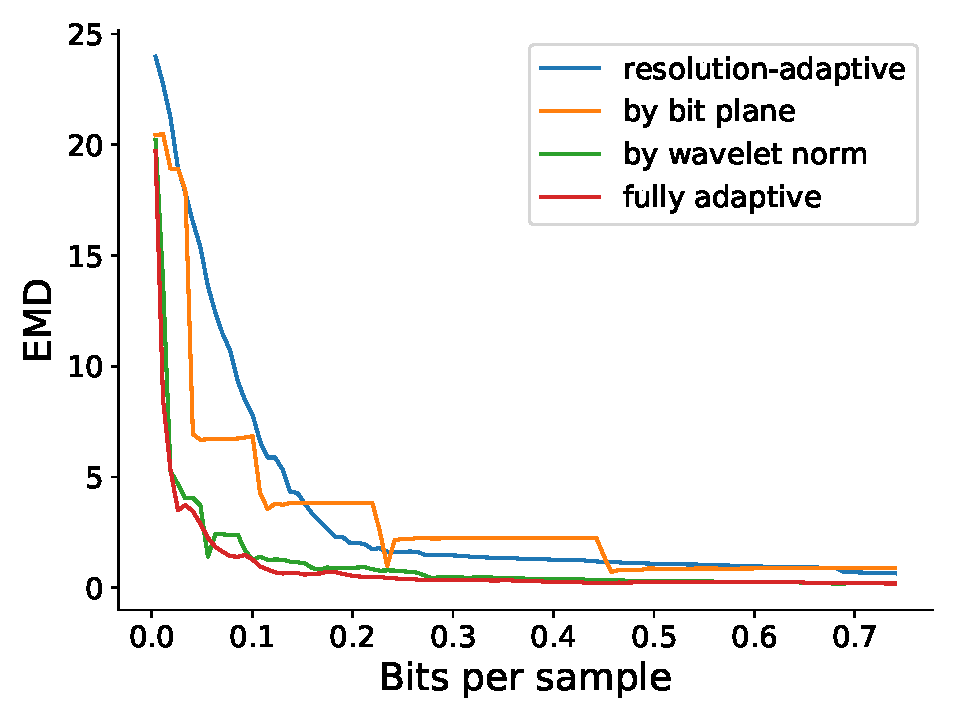
\includegraphics[width=0.44\linewidth]{img/motivation/boiler-histogram-motivation.pdf}}
	\subcaptionbox{Flame-OH}
	{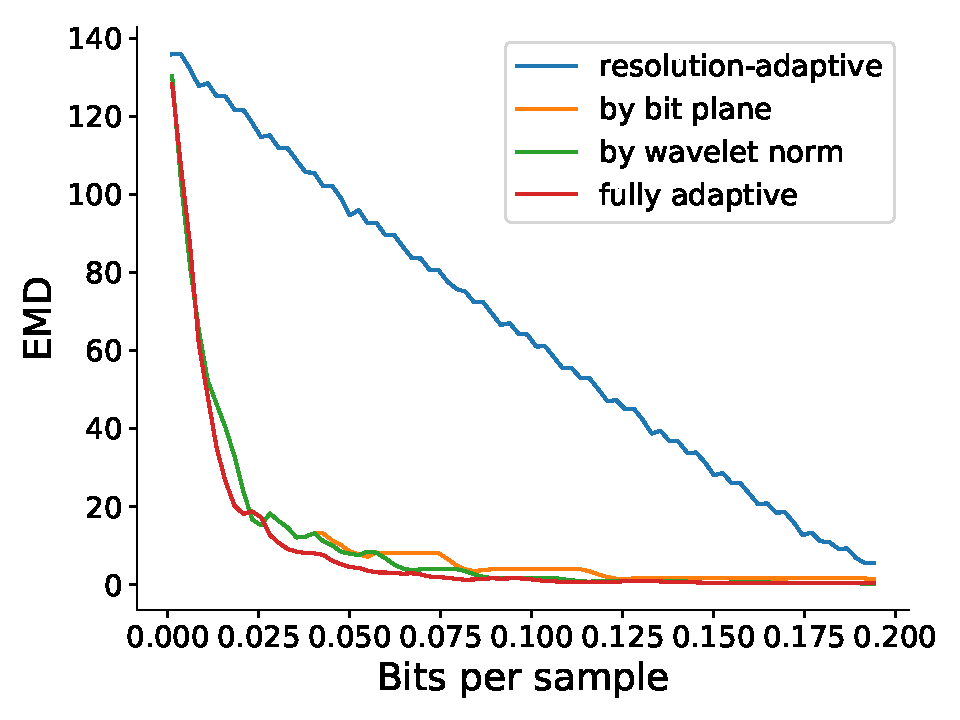
\includegraphics[width=0.44\linewidth]{img/motivation/kflame-oh-histogram-motivation.pdf}}
	\subcaptionbox{Miranda-diffusivity}
	{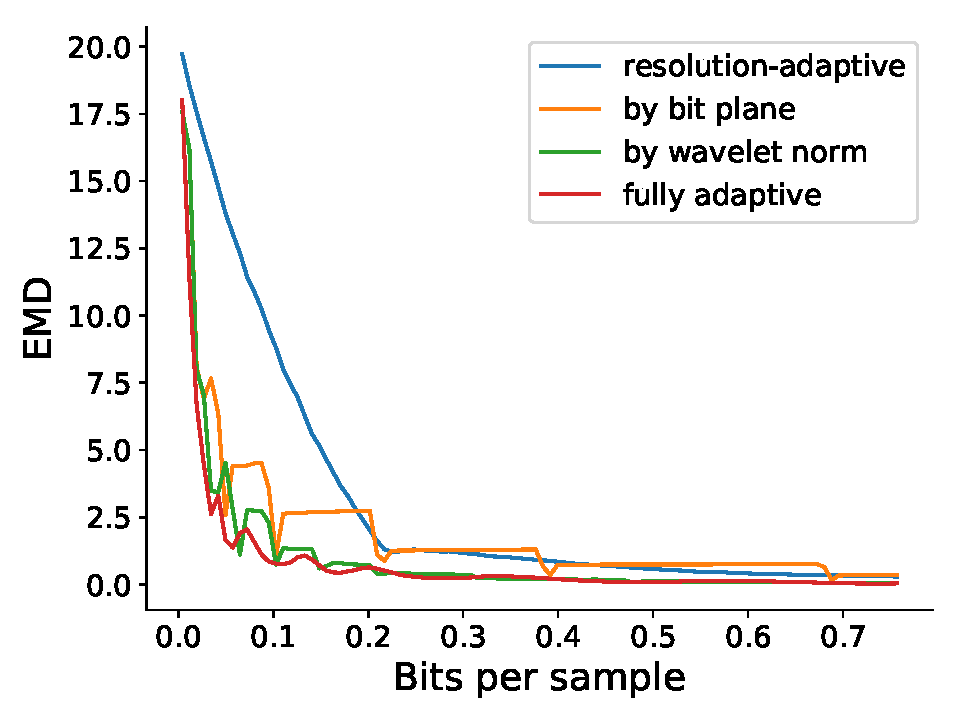
\includegraphics[width=0.44\linewidth]{img/motivation/diffusivity-histogram-motivation.pdf}}
	\caption{Histogram error comparison. Lower EMD is better. The streams are truncated	towards the
	end where the errors become negligibly small.}
	\label{fig:histogram-motivation}
\end{figure}

The \emph{by bit plane} and \emph{by wavelet norm} streams match one another closely in terms of
PSNR, but differ significantly in EMD. Furthermore, the \emph{fully adaptive, RMSE-optimized} stream
underperforms  \emph{fully adaptive, EMD-optimized}, indicating that recontructing an accurate
function and reconstructing an accurate histogram require two very different orderings of bits.
Figure \ref{fig:histogram-comparison} illustrates how a quantitative difference in EMD translates to
a visual difference in histogram.

\begin{figure}
	\centering
	\subcaptionbox{\emph{by bit plane}}
	{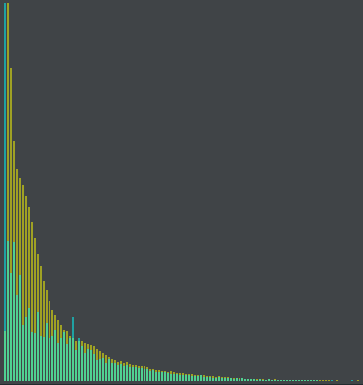
\includegraphics[width=0.24\linewidth]{img/motivation/histogram-by-bit-plane.png}}
	\subcaptionbox{\emph{by wavelet norm}}
	{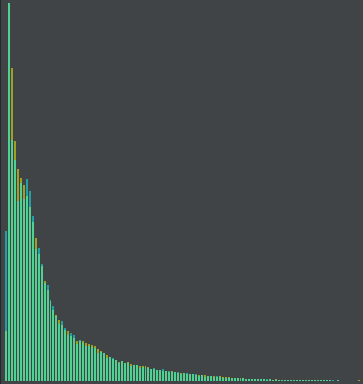
\includegraphics[width=0.24\linewidth]{img/motivation/histogram-by-wavelet-norm.png}}
	\subcaptionbox{\emph{fully adaptive, RMSE-optimized}}
	{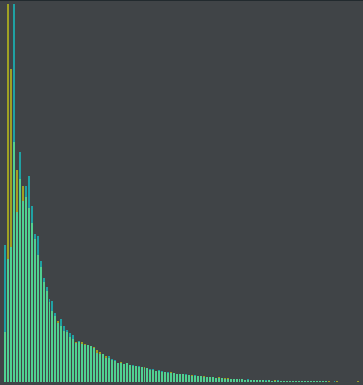
\includegraphics[width=0.24\linewidth]{img/motivation/histogram-rmse-optimized.png}}
	\subcaptionbox{\emph{fully adaptive, EMD-optimized}}
	{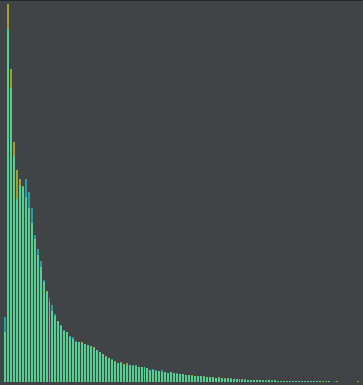
\includegraphics[width=0.24\linewidth]{img/motivation/histogram-emd-optimized.png}}
	\caption{Histogram comparison for the Magnetic data set at 0.16 bits per sample. The reconstructed
	histogram (blue) is blended with the groundtruth histogram (yellow), so green is where the two
	overlap. Larger overlap (more green, less blue and yellow) is better.}
	\label{fig:histogram-comparison}
\end{figure}

% \begin{figure}[htb!]
% 	\centering
% 	\subcaptionbox{without skip leading zeros}
% 	{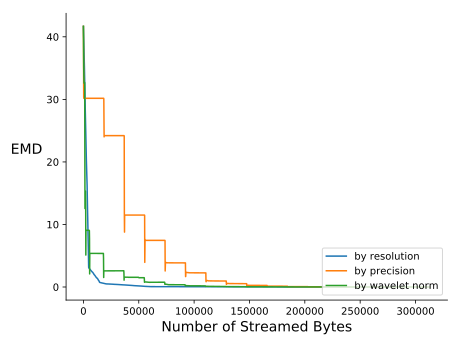
\includegraphics[width=0.4\linewidth]{img/independent/normalized/histogram-miranda-viscosity}}
% 	\subcaptionbox{with skip leading zeros}
% 	{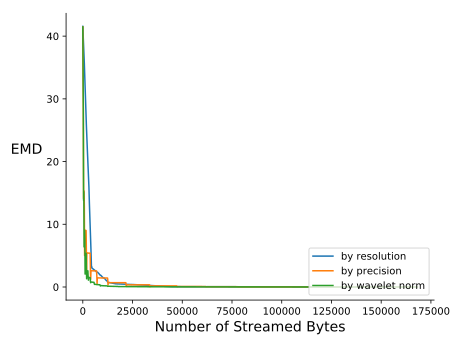
\includegraphics[width=0.4\linewidth]{img/skip-zeros/histogram-miranda-viscosity}}
% 	\caption {Histogram with earth mover distance (EMD) comparison between three streams: by bit-plane, by level, and by wavelet norm}
% 	\label{fig:histogram_traditional_vs_by_norm_viscosity}
% \end{figure}

% \begin{figure}[htb!]
% 	\centering
% 	\subcaptionbox{without skip leading zeros}
% 	{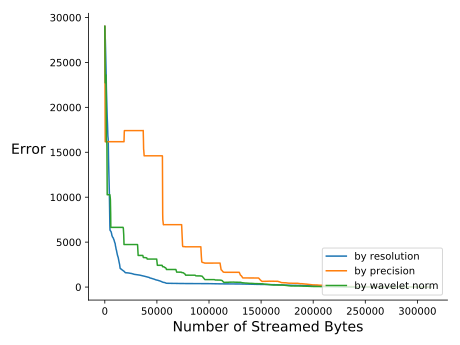
\includegraphics[width=0.4\linewidth]{img/independent/normalized/isocontour-miranda-viscosity}}
% 	\subcaptionbox{with skip leading zeros}
% 	{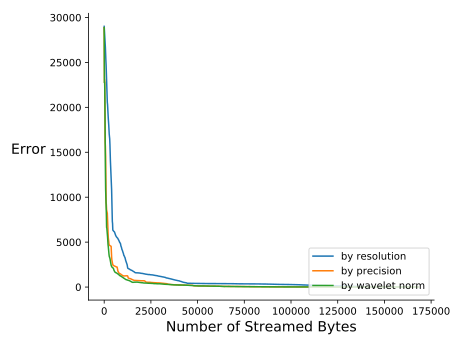
\includegraphics[width=0.4\linewidth]{img/skip-zeros/isocontour-miranda-viscosity}}
% 	\caption {Isocontour ($h = 0.0634$) comparison between three streams: by bit-plane, by level, and by wavelet norm}
% 	\label{fig:isocontour_traditional_vs_by_norm_viscosity}
% \end{figure}

% \begin{figure}
%   \centering
%   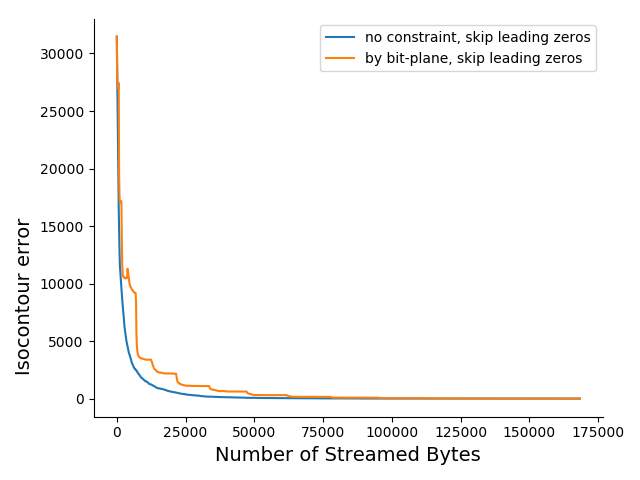
\includegraphics[width=0.8\linewidth]{resources/isocontour-error-by-bit-plane-viscosity.png}
%   \caption {By bit-plane isocontour comparison versus no constraints for viscosity, isoval=-0.005}
%   \label{fig:by_bit_plane_isocontour}
% \end{figure}
